% WebContactsProPlus — sequence: login + JWT cookie issuance
\documentclass[border=14pt]{standalone}
\usepackage{tikz}
\usetikzlibrary{positioning, arrows.meta, calc, fit}

\begin{document}
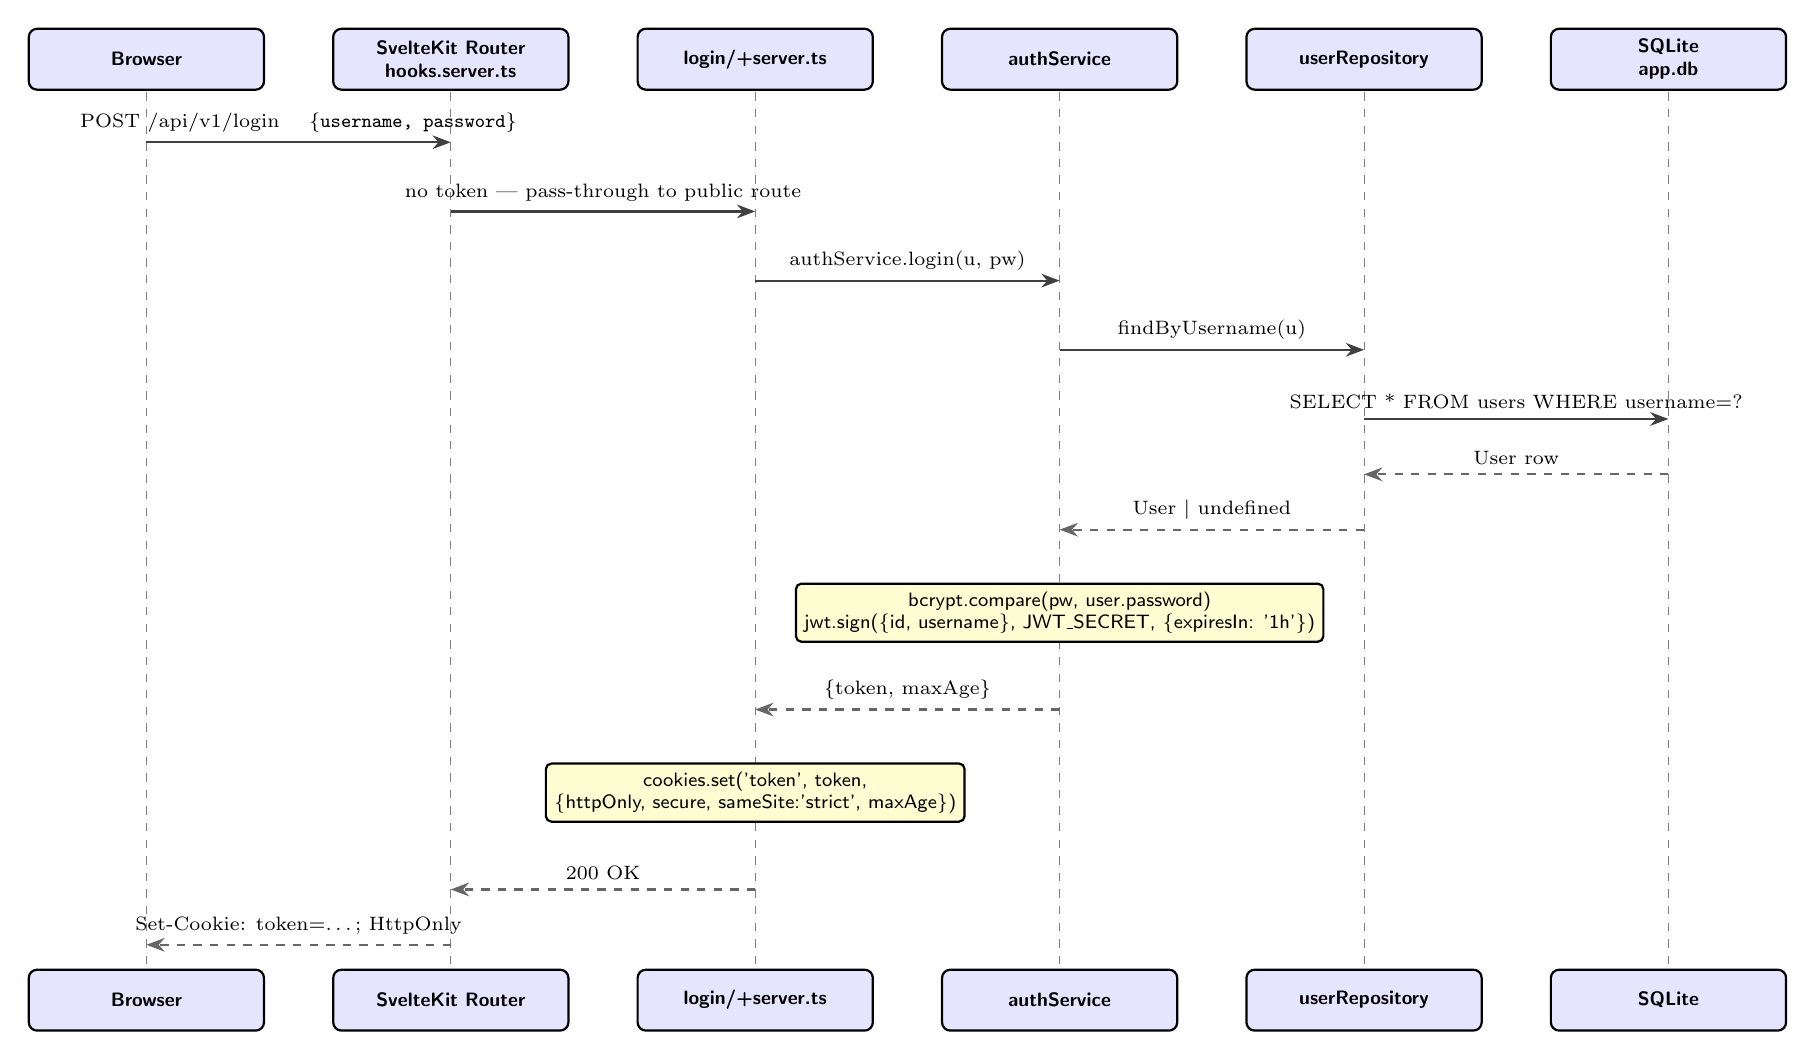
\begin{tikzpicture}[
    >=Stealth,
    font=\sffamily\footnotesize,
    actor/.style={
        draw, thick, fill=blue!10, rounded corners=3pt,
        minimum width=85pt, minimum height=22pt,
        align=center, font=\sffamily\scriptsize\bfseries,
    },
    msg/.style={->, thick, draw=black!75},
    ret/.style={->, thick, draw=black!60, dashed},
    note/.style={
        draw, thick, fill=yellow!18,
        rounded corners=2pt, align=center,
        font=\sffamily\scriptsize, inner sep=3pt,
    },
    lifeline/.style={dashed, draw=black!50},
    activation/.style={fill=blue!25, draw=blue!50, thick},
]

% column x-coordinates
\def\colA{0}     % Browser
\def\colB{110}   % SvelteKit router
\def\colC{220}   % login/+server.ts
\def\colD{330}   % authService
\def\colE{440}   % userRepository
\def\colF{550}   % SQLite

% participants (top)
\node[actor] (A) at (\colA pt,0)   {Browser};
\node[actor] (B) at (\colB pt,0)   {SvelteKit Router \\ {\scriptsize hooks.server.ts}};
\node[actor] (C) at (\colC pt,0)   {login/+server.ts};
\node[actor] (D) at (\colD pt,0)   {authService};
\node[actor] (E) at (\colE pt,0)   {userRepository};
\node[actor] (F) at (\colF pt,0)   {SQLite \\ {\scriptsize app.db}};

% lifelines
\def\bot{-340pt}
\foreach \x in {\colA, \colB, \colC, \colD, \colE, \colF}
    \draw[lifeline] (\x pt,-12pt) -- (\x pt,\bot);

% participants (bottom mirror)
\node[actor] at (\colA pt, \bot)   {Browser};
\node[actor] at (\colB pt, \bot)   {SvelteKit Router};
\node[actor] at (\colC pt, \bot)   {login/+server.ts};
\node[actor] at (\colD pt, \bot)   {authService};
\node[actor] at (\colE pt, \bot)   {userRepository};
\node[actor] at (\colF pt, \bot)   {SQLite};

% --- messages ---
\draw[msg]  (\colA pt,-30pt) -- node[above, font=\scriptsize] {POST /api/v1/login \quad \texttt{\{username, password\}}} (\colB pt,-30pt);
\draw[msg]  (\colB pt,-55pt) -- node[above, font=\scriptsize] {no token — pass-through to public route} (\colC pt,-55pt);
\draw[msg]  (\colC pt,-80pt) -- node[above, font=\scriptsize] {authService.login(u, pw)} (\colD pt,-80pt);
\draw[msg]  (\colD pt,-105pt) -- node[above, font=\scriptsize] {findByUsername(u)} (\colE pt,-105pt);
\draw[msg]  (\colE pt,-130pt) -- node[above, font=\scriptsize] {SELECT * FROM users WHERE username=?} (\colF pt,-130pt);
\draw[ret]  (\colF pt,-150pt) -- node[above, font=\scriptsize] {User row} (\colE pt,-150pt);
\draw[ret]  (\colE pt,-170pt) -- node[above, font=\scriptsize] {User \textbar{} undefined} (\colD pt,-170pt);

% note: bcrypt + JWT sign
\node[note] (n1) at (\colD pt,-200pt) {
    bcrypt.compare(pw, user.password) \\
    jwt.sign(\{id, username\}, JWT\_SECRET, \{expiresIn: '1h'\})
};

\draw[ret]  (\colD pt,-235pt) -- node[above, font=\scriptsize] {\{token, maxAge\}} (\colC pt,-235pt);

% note: cookies.set
\node[note] (n2) at (\colC pt,-265pt) {
    cookies.set('token', token, \\ \{httpOnly, secure, sameSite:'strict', maxAge\})
};

\draw[ret]  (\colC pt,-300pt) -- node[above, font=\scriptsize] {200 OK} (\colB pt,-300pt);
\draw[ret]  (\colB pt,-320pt) -- node[above, font=\scriptsize] {Set-Cookie: token=\dots; HttpOnly} (\colA pt,-320pt);

\end{tikzpicture}
\end{document}
